\chapter{Fundamentals}
\label{chap:fundamentals}

Under the term \emph{ray tracing} we understand the utilization of algorithms that involve the casting of virtual light rays for generating images. The purpose of these light rays is to archive high visual realism by the simulation of real-life behavior.

We as persons can perceive nearby objects or persons due to the following: Light sources, either natural or artificial, emit electromagnetic (EM) waves. This radiation is reflected off objects in the scene (informally, it "bounces" on objects). The human eye or a camera sensor interprets EM waves of different frequencies as colors. The resulting transport of these EM waves in the scene to the human eye or a camera sensor forms an image.

The purpose of ray tracing algorithms is to imitate this behavior, usually by tracing these light rays in reverse order from a point in the scene, a virtual camera or an "eye point", back to the emitting light source.

\begin{figure}[h]
	\centering
	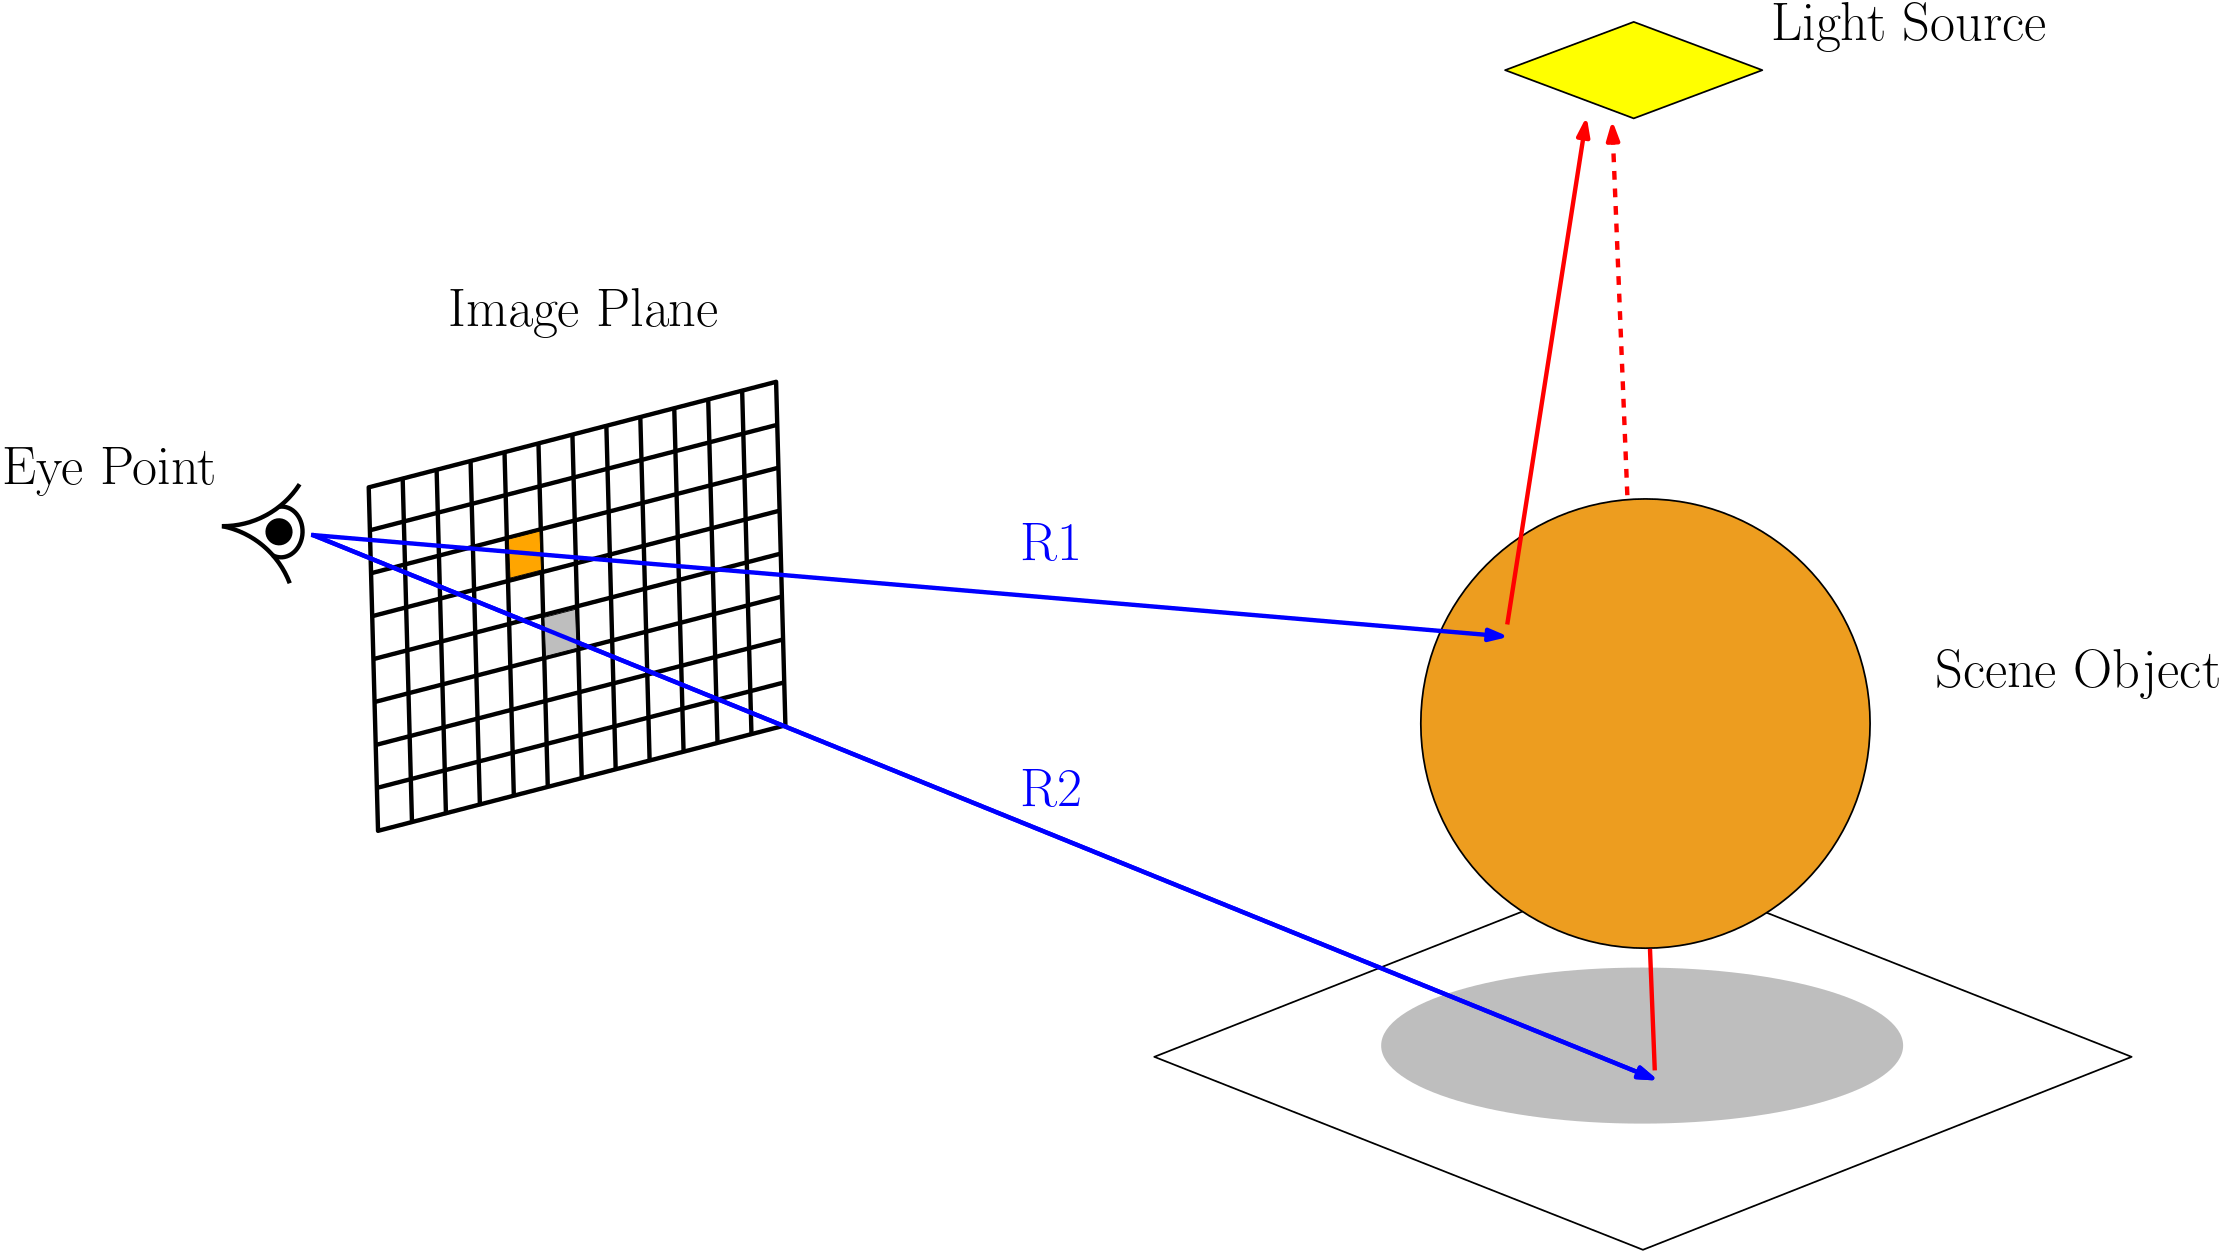
\includegraphics[width=.9\linewidth]{img/1 fundamentals/ray_tracing.png}
	\caption{Ray tracing procedure for calculating global illumination.}
	\label{fig:raytracer_general}
\end{figure}

An advantage of these ray tracing algorithms is its core procedure being straightforward when viewed from a theoretical point of view. 

Figure \ref{fig:raytracer_general} shows an example of a virtual scene. It is composed of an orange sphere, a white ground plane, and a light source. Furthermore, an image plane exists in the scene, on which the 2D image of the 3D scene will be projected. 
A ray is consisting of two components, an origin point and a direction vector. The $Eye Point$ in \ref{fig:raytracer_general} will serve as the origin of the cast rays. In the figure, the image plane is composed of multiple quadratic "cells" that represent the actual pixels of the resulting image. Through each of these cells, a ray is cast into the scene from the eye point. 

The subsequent step is to determine, whether that ray intersected a particular geometry by performing intersection tests on all geometries in the scene \footnote{Testing all geometries present in a complex scene for intersection is of course a naive approach and not practical at all. This procedure is solely mentioned here for the sake of illustration. Section \ref{sec:acceleration} introduces some common ray acceleration data structures to compensate for this.}. 

In case a geometry is intersected, a secondary ray is generated with its origin at the intersection point with the closest distance to the $Eye Point$ and its direction toward the light source. In case this secondary light ray does not intersect any other geometry between its origin and the light source, this means that the first intersection point is exposed to light and the material color at that point is used for the corresponding pixel (see R1 in figure \ref{fig:raytracer_general}). Otherwise, the intersection point must be in shadow (see R2). This procedure generates an image with local illumination.

The following chapter is dedicated to providing background information on ray tracing, shape representation in rendering systems, and ray acceleration data structures. Furthermore, the Embree framework is introduced.

\section{Ray tracing algorithms}

The following section outlines the development of various ray tracing techniques. The pioneering work of \cite{appel1968some} and \cite{whitted1979improved} will be briefly discussed. Furthermore, the derivation from the definition of radiance to the rendering equation \cite{kajiya1986rendering}, whose numerical solving via Monte Carlo integration is the purpose of modern rendering environments, will be presented.

\subsection{Origins of ray tracing}
As briefly mentioned in the Introduction, ray tracing was pioneered in 1968 by \cite{appel1968some}. His work aimed to provide basic shading for wire-framed solids to communicate better spatial relations and depth of objects in the rendered image.

To achieve this shading, virtual light rays were cast from a scene light source in random directions. Whenever one such ray intersects a geometry, a character or symbol (e.g., a small "plus"-symbol or square) was placed at that intersection point. If enough rays were cast, areas on the solid exposed to light would be shaded by these symbols.
The result would then come to be by inverting the shaded and non-shaded areas of the geometry.

\begin{figure}
	\centering
	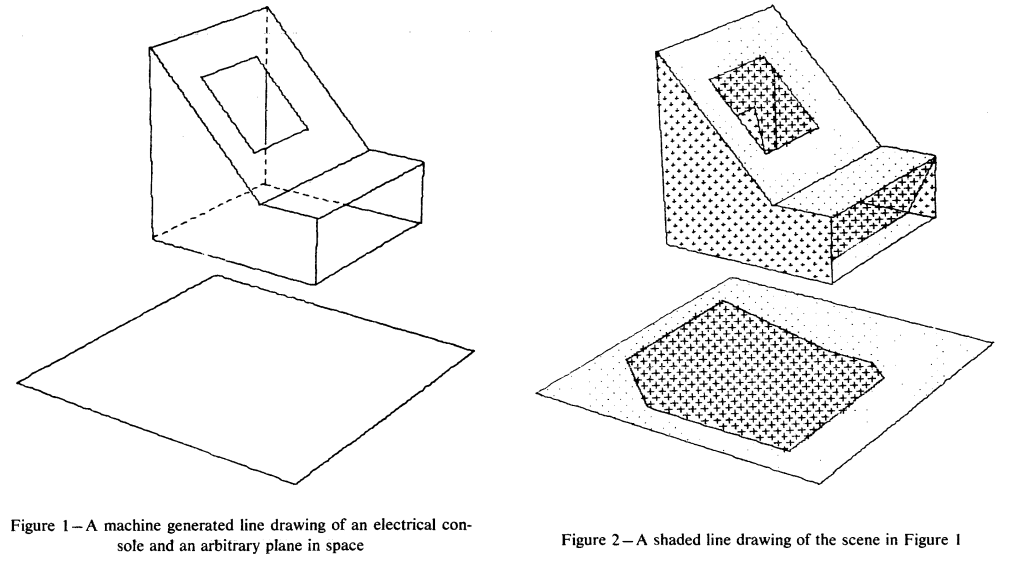
\includegraphics[width=1\linewidth]{img/1 fundamentals/appel_comp}
	\caption{Original figures from \cite{appel1968some}. The left figure shows plain solid geometry and the right figure shows the same solid with shading applied to it.}
	\label{fig:appel_paper}
\end{figure}

Figure \ref{fig:appel_paper} shows a result of this approach. Without the additional shading information, it would be difficult for the observer to perceive the position of the upper geometry relative to the plane. To achieve convincing results, a high number of rays had to be generated ("Even for about 1000 light rays, results were splotchy." \cite[p 3]{appel1968some}). At the time of publication, the available hardware was hardly powerful enough for this shading method.

The idea of casting rays later became a key utilization for a shading model that aimed for higher realism by taking the "global setting" of geometries into account \cite{whitted1979improved}. A variety of shading models existed at that time, which was able to display optical effects convincingly. However, these models usually worked only in special cases and not well with each other, as noted by Andrew Glassner in the preface of his book \citetitle{glassner1989introduction} \cite{glassner1989introduction}. For example, some models existed that were good at calculating reflection effects but could not handle refraction effects well. And vice versa. 

\cite{whitted1979improved} introduced a shading model that would truthfully simulate reflection, shadows and refraction as well as the effects of other conventional shading models at that time.  
The model is partially derived from an empirical reflection model developed by \cite{phong1975illumination}. This so-called "Phong reflection model" assumes that light, which is reflected from a surface, is composed of ambient reflection, diffuse reflection and specular reflection.
In contrast, Whitted's model assumes that the light intensity arriving at the $Eye Point$ from an intersection point is conglomerated by a specular reflection component and a transmission component. 

In real-life, light that is propagated towards an observer from a surface most certainly has interacted with other surfaces before. If true realism of computer generated images is desired, these previous interactions have to be taken into consideration, even for virtual scenes with moderately complex geometry. An example of such an event can be seen in Figure \ref{fig:whitted_rays}.

\begin{figure}
	\centering
	\subfloat[Light is being reflected from other surfaces before reaching the Eye Point.]{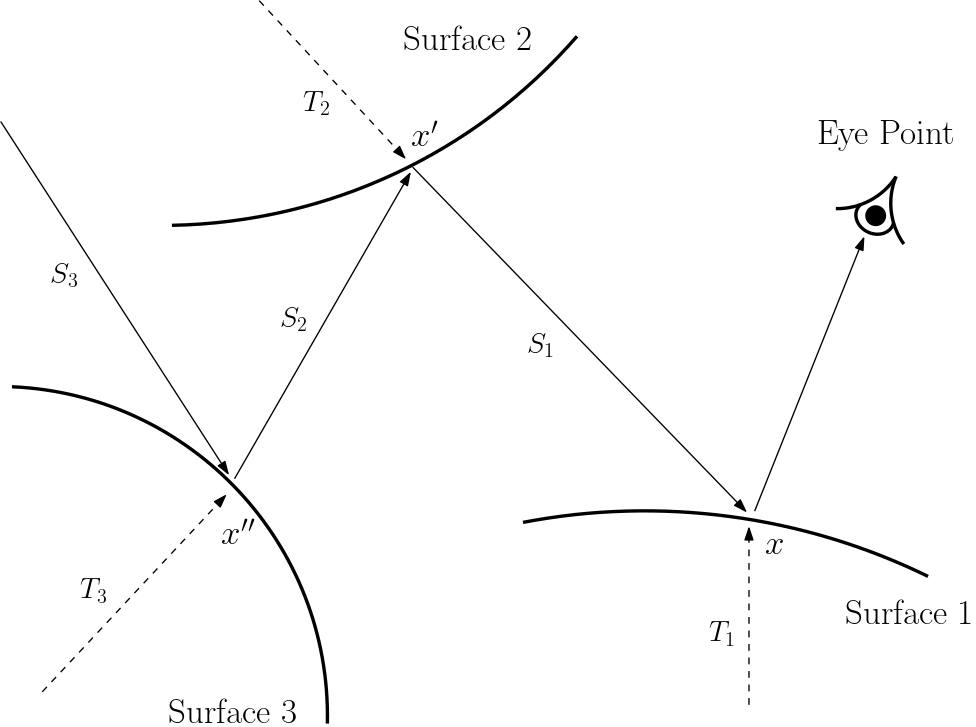
\includegraphics[width=.6\textwidth]{img/1 fundamentals/whitted_rays.png}\label{fig:whitted_rays}}
	\hfill
	\subfloat[Tree structure storing the individual reflection and transmission components.]{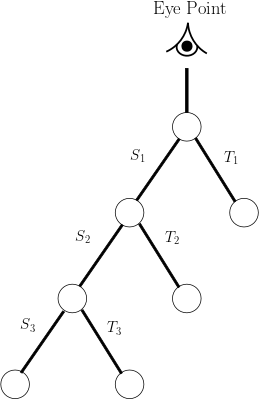
\includegraphics[width=.3\textwidth]{img/1 fundamentals/whitted_tree.png}\label{fig:whitted_tree}}
	\caption{Figures based on the original figures from the paper \citetitle{whitted1979improved} \cite{whitted1979improved}}
\end{figure}

This natural behavior is implemented in the following way. From the $Eye Point$, a ray is cast towards the virtual scene and a possible intersection point $x$ with the scene geometry is calculated. 
The transmission and specular component rays at that intersection point are then recursively calculated and stored in a tree data structure which is shown in Figure \ref{fig:whitted_tree}. 
To prevent a branch of the tree from growing infinitely large, it is truncated as soon as an attempt is made to access more storage than was previously made available for it. After such a tree is created, it is traversed recursively in order to calculate the light intensity at each node, finally resulting in the calculation of the total light intensity that is reflected towards the $Eye Point$. Between two nodes, the intensity is attenuated according to a distance function between the intersection points, associated with the node and the node's parent node. 
Such trees are created and traversed for every pixel of the image plane. This procedure allows for the convincing display of a variety of optical effects with the help of a single model.

\subsection{The Rendering Equation}

\begin{figure}
	\centering
	\subfloat[]{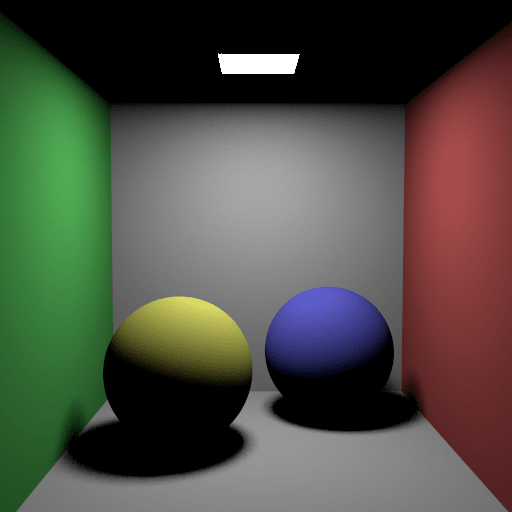
\includegraphics[width=.4\textwidth]{img/1 fundamentals/cb_direct.png}\label{fig:cb_local}}
	\hfil
	\subfloat[]{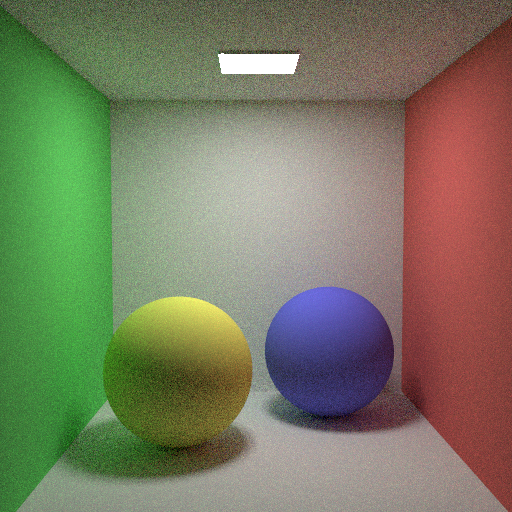
\includegraphics[width=.4\textwidth]{img/1 fundamentals/cb_global.png}\label{fig:cb_global}}
	\caption{The Cornell Box scene with direct illumination (Figure \ref{fig:cb_local}) and global illumination (Figure \ref{fig:cb_global}). Both scenes were rendered by a simple ray tracing program that was implemented by students attending the course \citetitle{cg3}, held at Charles University in Prague \cite{cg3}.}
\end{figure}

Figure \ref{fig:cb_local} shows an image of the Cornell Box. The scene's appearance results from shooting a ray into the scene, calculating a possible intersection point, and then generating a second ray in the direction of the light source. However, the appearance of the Cornell Box is not physically realistic because the ceiling is not illuminated. This is since, with this approach, no light rays that interact with surface points on the ceiling can directly reach the emissive area of the light source. The degree of realism of the scene shown in Figure \ref{fig:cb_local} can be significantly improved by considering global illumination effects. 

In 1986, an integral equation was developed by Kajiya \cite{kajiya1986rendering}, that would describe the total reflected radiance towards an observer as the "sum" (or integral) of all light contributions over a hemisphere at a point on a surface. This mathematical model takes direct illumination (light from light sources) and indirect illumination (light being reflected off other surfaces in the scene) into account.
\\

The so-called \emph{Rendering Equation} is given by

\begin{equation}\label{eq:renderingeq}
L(x, \omega_{o}) = L_{e}(x, \omega_{o}) + \int_{H(x)} L(x, \omega_{i})f_{r}(\omega_{i} \rightarrow \omega_{o})\cos\theta\partial\omega_{i}
\end{equation}

\noindent where
\begin{itemize}
	\setlength\itemsep{0.05em}
	\item  $L(x, \omega_{o})$ is the total reflected light intensity from a surface point $x$ towards the observer along the outgoing direction $\omega_{o}$,
	\item  $L_{e}(x, \omega_{o})$ is the radiance emitted at the surface point $x$ and propagated along $\omega_{o}$,
	\item  $H(x)$ is a hemisphere over surface point $x$,
	\item 	$L(x, \omega_{i})$ is the light intensity incident to $x$ along direction $\omega_{i}$, 
	\item  $f_{r}(\omega_{i} \rightarrow \omega_{o})$ is the Bidirectional Reflectance Distribution Function (BRDF), and 
	\item  $\cos\theta$ is a term, compensating for Lambert's cosine law.
\end{itemize}

For a better understanding of the individual terms of the rendering equation, a definition of radiance and a brief explanation of the bidirectional reflectance distribution function and the local reflection equation is provided in the following subsections.
The information provided by these subsections are collated from the lecture notes of the course \citetitle{cg3} held at Charles University in Prague, Czech Republic \cite{cg3}, from the book \citetitle{pharr2016physically} \cite{pharr2016physically} and from the book \citetitle{hughesDamEtAl13} \cite{hughesDamEtAl13}.

\subsubsection{Definition of radiance}

We define the \emph{radiance} of a source, sometimes informally referred to as "brightness", as the power per unit area $\partial A$ perpendicular to the ray in the direction $\omega_{o}$ and per unit solid angle that is propagated along with it (see Figure \ref{fig:radiance}). The following equation describes this:

\begin{equation}
L(\omega_{o}) = \frac{\partial^2\phi}{\partial\omega_{o}\partial A\cos\theta} [\mathrm{W}\cdot \mathrm{sr}^{-1}\cdot \mathrm{m}^{-2}]
\end{equation}

\noindent where
\begin{itemize}
	\setlength\itemsep{0.05em}
	\item  $\omega_{o}$ is the outgoing direction
	\item  $\phi$ is flux or radiance per unit time
	\item  $A$ is the surface area, and
	\item  $\cos\theta$ a term for compensating Lambert's cosine law
\end{itemize}

\begin{figure}
	\centering
	\subfloat[Radiance is defined as the radiant flux emitted, received or reflected per solid angle $\partial\omega_{o}$ per unit projected area $\partial A$.]{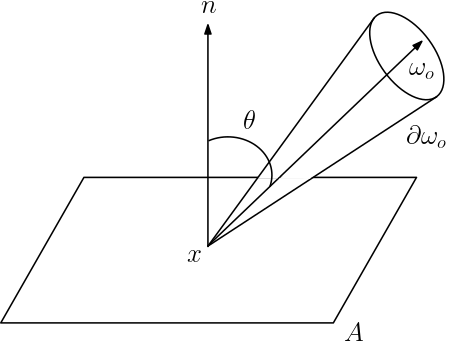
\includegraphics[width=.4\textwidth]{img/1 fundamentals/radiance.png}\label{fig:radiance}}
	\hfill
	\subfloat[The BRDF is a function defining how much light from the incoming direction$\omega_{i}$ is reflected towards the viewer along the outgoing direction $\omega_{o}$.]{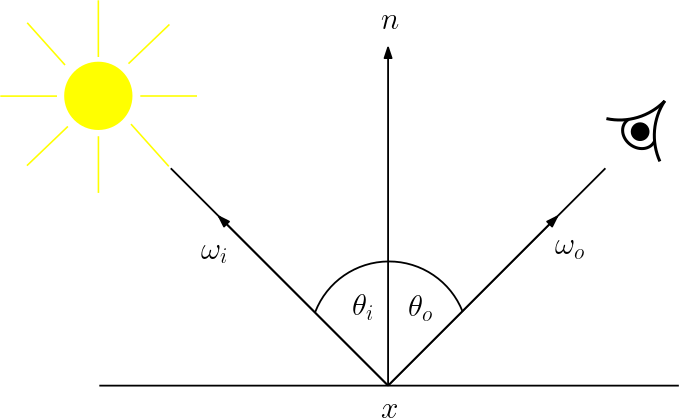
\includegraphics[width=.5\textwidth]{img/1 fundamentals/brdf.png}\label{fig:brdf}}
	\caption{Diagrams visualizing radiance (Figure \ref{fig:radiance}) and the BRDF (Figure \ref{fig:brdf}).}
\end{figure}

From this definition we can derive the bidirectional reflectance distribution function.

\subsubsection{Bidirectional Reflectance Distrubution Function (BRDF)}
The \emph{Bidirectional Reflectance Distribution Function (BRDF)} is a mathematical model describing the reflection properties of a given surface. To be precise, it describes the probability of light energy, arriving at a point $x$ on a surface from direction $\omega_{i}$, being reflected along the reflection $\omega_{o}$. 
The BRDF model is defined by:

\begin{equation} \label{eq:brdf}
f_{r}(\omega_{i} \rightarrow \omega_{o}) = \frac{\partial L_{r}(\omega_{o})}{L_{i}(\omega_{i})\cos\theta\partial\omega_{i}} [\mathrm{sr}^{-1}]
\end{equation}

\noindent where
\begin{itemize}
	\setlength\itemsep{0.05em}
	\item  $L_{r}(\omega_{o})$ is the reflected light energy from a surface point along the direction $\omega_{o}$, and
	\item  $L_{i}(\omega_{i})$ is the incident light energy arriving at the surface point from direction $\omega_{i}$ 
\end{itemize}

Properties of BRDFs are the conservation of energy and the Helmholtz reciprocity, which considers the incident and reflected light intensities in Equation \ref{eq:brdf} as interchangeable without affecting the result. There exist different types of BRDFs: empirical BRDFs, physically based BRDFs, and BRDFs being an approximation of measured data.
BRDFs are a crucial component when calculating direct illumination with the \emph{local reflection equation}.

\subsubsection{Reflection Equation}

The \emph{Reflection Equation} describes how much total light is reflected from a surface point $x$ towards an observer along a given direction $\omega_{o}$, taking the light intensities arriving at $x$ from all incident directions into account. It is given by:

\begin{equation}\label{eq:local}
L_{r}(x, \omega_{o}) = \int_{H(x)} L_{i}(x, \omega_{i})f_{r}(\omega_{i} \rightarrow \omega_{o})\cos\theta\partial\omega_{i}
\end{equation}

\noindent where
\begin{itemize}
	\setlength\itemsep{0.05em}
	\item $H(x)$ is a hemisphere over the surface point $x$.
\end{itemize}
The total amount of reflected energy is calculated by integrating all contributions of incident radiance over the hemisphere $H(x)$. The BRDF serves as a weight in this equation because only the energy reflected along $\omega_{o}$ is considered.
 
\subsubsection{The Rendering Equation revisited}

The rendering equation, which for reasons of convenience is shown again in Equation \ref{eq:renderingeq2} can be arguably regarded as an extension of the local reflection equation.

\begin{equation}\label{eq:renderingeq2}
L(x, \omega_{o}) = L_{e}(x, \omega_{o}) + \int_{H(x)} L(x, \omega_{i})f_{r}(\omega_{i} \rightarrow \omega_{o})\cos\theta\partial\omega_{i}
\end{equation}

Essentially, it describes the total reflection of energy towards direction $\omega_{o}$ from a surface point $x$ as the "sum" or integral of all the light intensity, incident to all directions over a hemisphere over the point $x$, together with the intensity emitted from point $x$, if $x$ is located on an emissive material. The unknown variable $L$ is present on both sides of this equation.

This function is a higher-order integral which is difficult to solve analytically. The most common approach to solving this integral equation is the utilization of Monte Carlo methods. Monte Carlo methods numerically approximate a given integral by drawing random samples. The convergence speed of this procedure is independent of the dimension of the integral. Most of today's image synthesis algorithms implement Monte Carlo methods to approximate the rendering equation's solution.



\subsubsection{Path tracing}

Multiple approaches for solving the rendering equation exist, for example, the \emph{radiosity method} \cite{goral1984modeling}, which aims at solving it via the application of the finite element method. However, the most commonly used techniques for solving the rendering equation are Monte Carlo methods.
The Monte Carlo method \emph{path tracing} This method is based on the property that in a vacuum, radiance is constant along straight lines.   

\begin{figure}
	\centering
	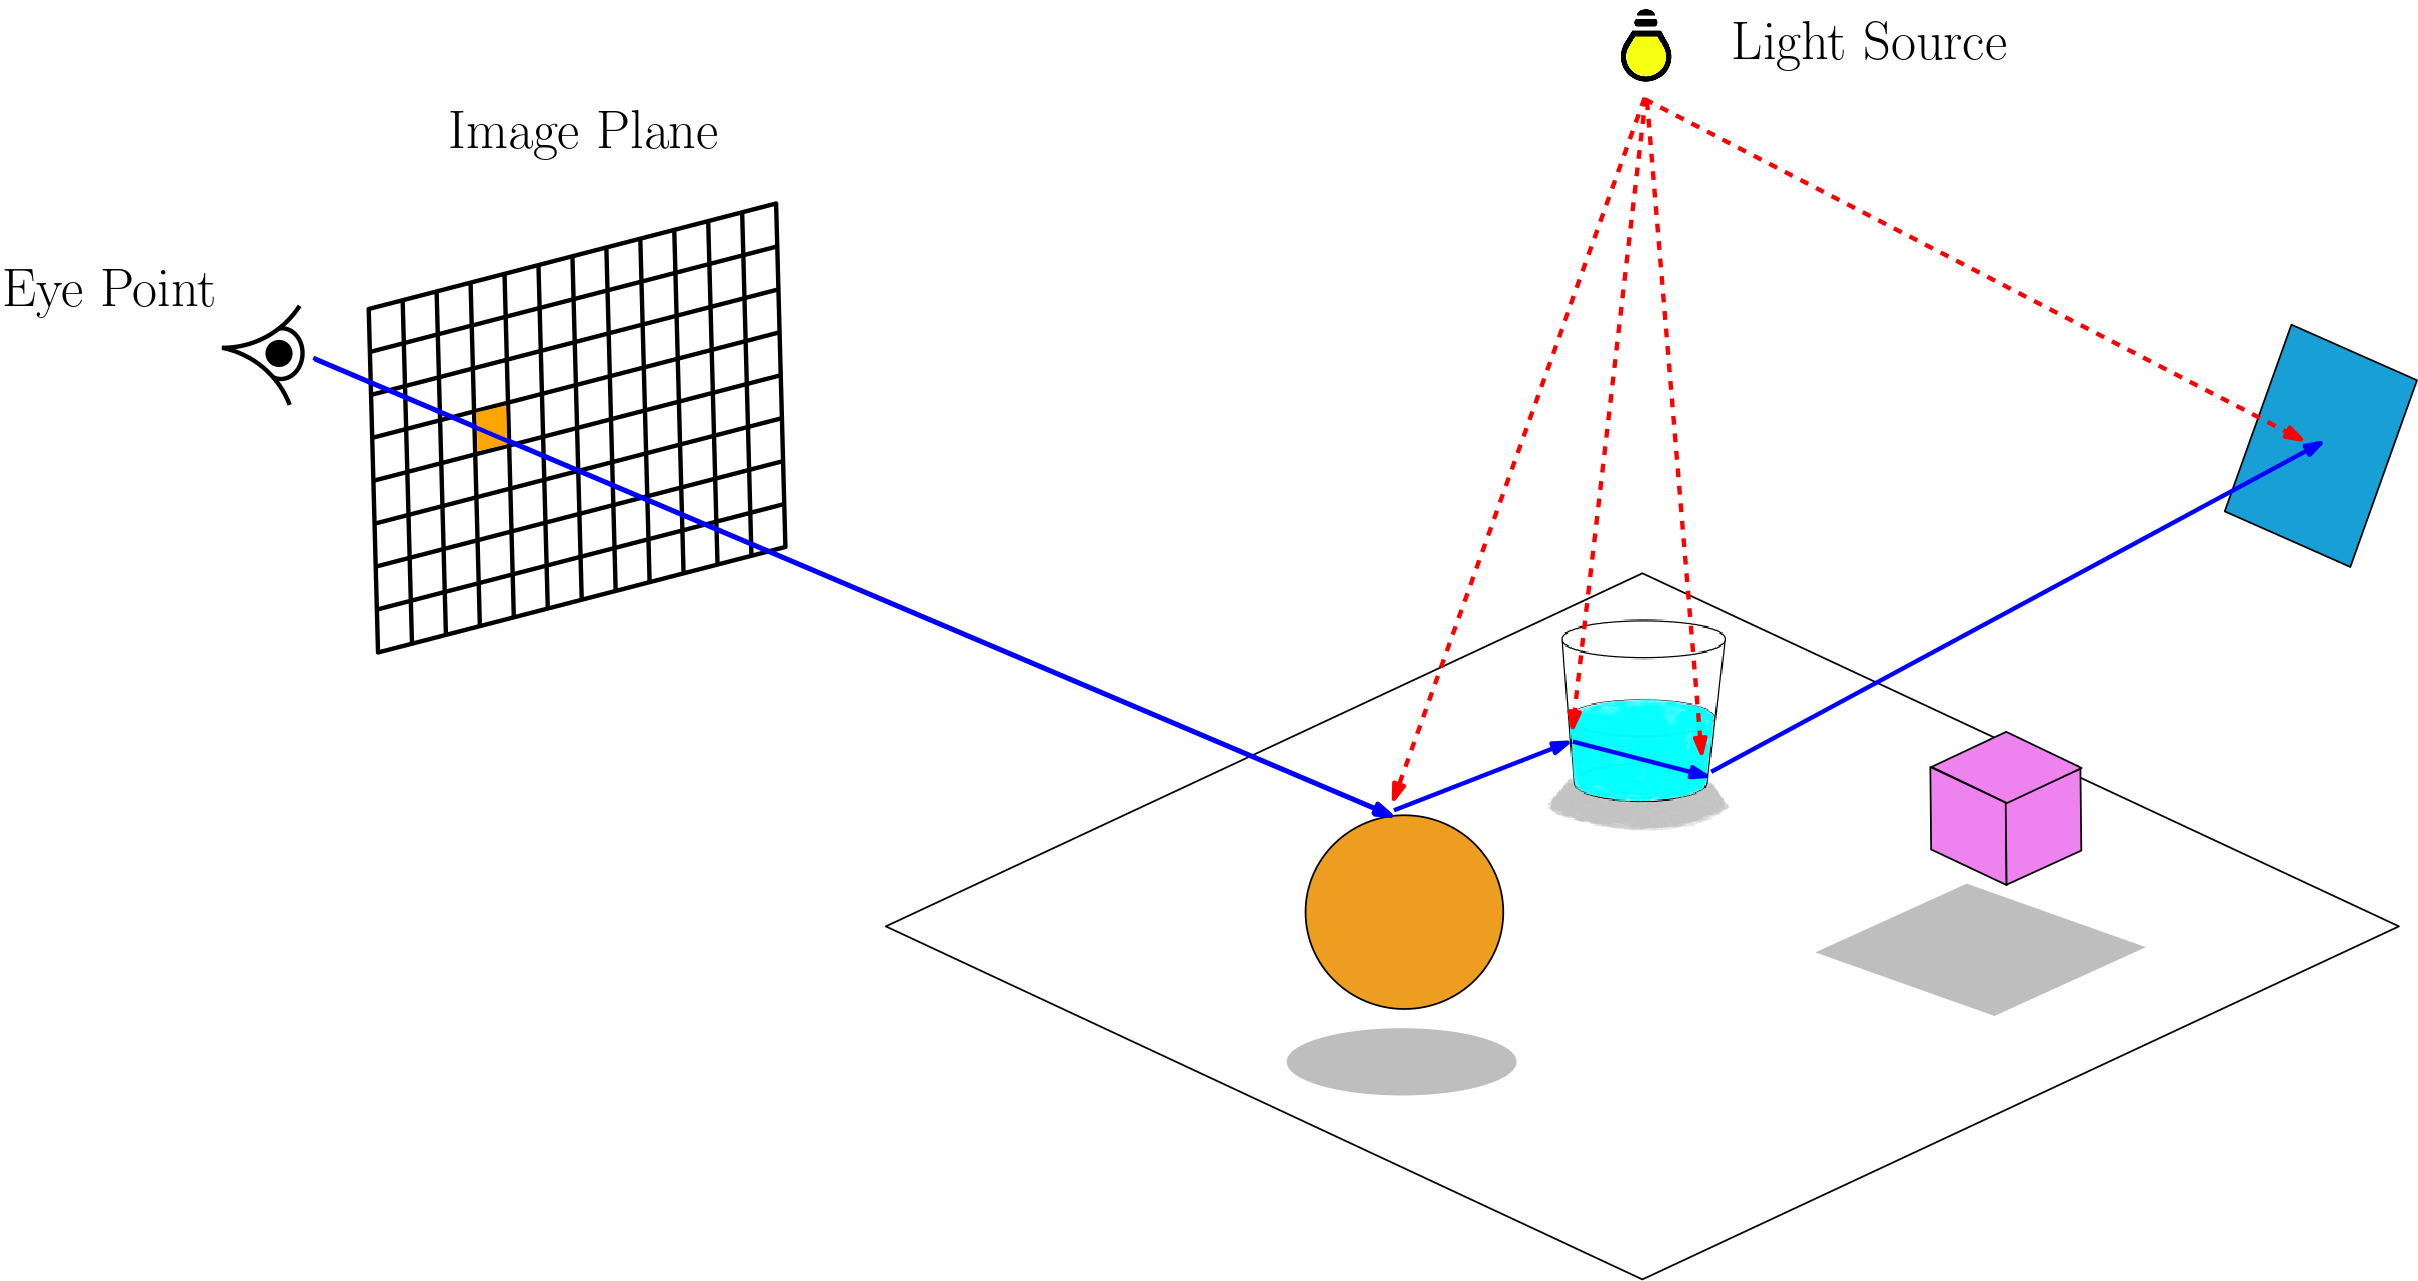
\includegraphics[width=1\linewidth]{img/1 fundamentals/path_tracing.png}
	\caption{Tracing a path for calculating global illumination.}
	\label{fig:pathtracing}
\end{figure}

When a given ray intersects scene geometry, a secondary ray can be spawned at the intersection point, going along a direction that conforms to the BRDF associated with the intersected geometry. By repetition of this procedure, a "path" of rays is generated.

To calculate light intensity at each pixel of an image, path tracing generates such paths of rays, starting at the $Eye Point$ and ending at a light source. An example of such a path is visualized in Figure \ref{fig:pathtracing}. At each intersection point along the path, the intersected geometries are tested for occlusion concerning the light sources available in the scene. If another geometry does not occlude the shape, the direct contribution of the light sources is accumulated.
To prevent the calculations of unprofitable paths, a path is continued according to a so-called "survival probability." This probability can, for example,  be formulated as the reflectivity of the surface, which is intersected by a ray. If this surface, for example, reflects only ten percent of light energy, the path is continued with a probability of then percent.
To approximate an integral part of the rendering equation, numerous paths are generated at the intersection point $x$. To generate the final color of the image pixels, the results calculated by the paths are averaged.

\begin{figure}
	\centering
	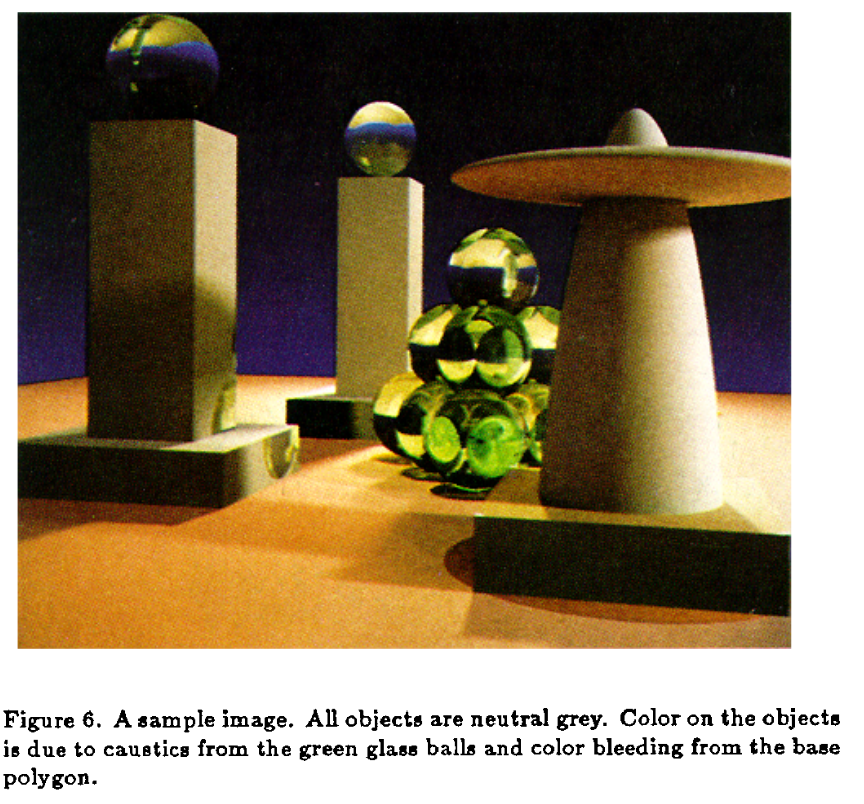
\includegraphics[width=.7\linewidth]{img/1 fundamentals/rendering_eq_figure.png}
	\caption{Original figure from \cite{kajiya1986rendering}.}
	\label{fig:kajiya_figure}
\end{figure}

Concerning path tracing, we can re-write the rendering equation shown in \ref{eq:renderingeq} in the following way:
\begin{equation}\label{eq:renderingeq_update}
L(x, \omega_{o}) = L_{e}(x, \omega_{o}) + \int_{H(x)} L(ray(x, \omega_{i}), -\omega_{i})f_{r}(\omega_{i} \rightarrow \omega_{o})\cos\theta\partial\omega_{i}
\end{equation}

The term $ray(x, \omega_{i})$ is a function for recursively calculating all incoming radiance arriving at the point $x$.

In comparison to the ray tracing method of \cite{whitted1979improved}, path tracing is capable of simulating advanced optical effects such as soft shadows and diffuse interreflection. An example of this can be seen in Figure \ref{fig:cb_global}.

\section{Solid representations in 3D space}

A crucial part of ray tracing algorithms is calculating intersection points between rays and the scene geometry.
Solid objects can be represented in the Euclidean space in various ways. The intersection testing for these solids will depend on their representation.

The following section illustrates three types of solid representations in image synthesis environments, such as ART: Analytic surfaces, polygon meshes, and constructive solid geometry.

\subsection{Analytical surfaces}
\label{sec:quadrics}
Analytical surfaces are surfaces in three-dimensional Euclidean space, defined by analytic functions. Common analytical surfaces are quadric shapes (or sometimes called quadrics). Examples of this type of surface representation are spheres, cones, cylinders, and paraboloids. The equations describing these shapes can be in implicit form, which has the pleasant property, that testing whether a point $p$ is located at the boundary of such a surface is easy. 

Generally speaking, implicit equations are relations of the form \\  $f(x_{0}, x_{1}, ..., x_{n-1}) = 0$ where $f$ is a function of multiple variables. These variables can be considered coordinates of a point $p$ in $n$-dimensional space and evaluated by function $f$. An evaluation of $f$ will result in two possible outcomes: either $f(p) = 0$, which means $p$ is located on the surface of the shape, or  $f(p) \ne 0$, which means the opposite.

Due to this straightforward evaluation, analytical shapes are well suited for intersection testing during ray tracing.

In the following, we will provide an example of an intersection calculation between a given unit sphere $S$ with radius $1$ and a given ray $R$. 

\begin{figure}
	\centering
	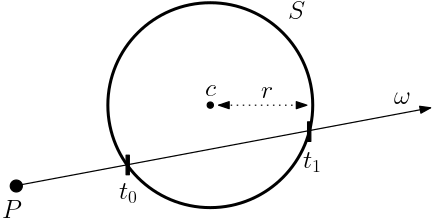
\includegraphics[width=.5\linewidth]{img/1 fundamentals/sphere_isect.png}
	\caption{Intersection between a sphere $S$ with its center point $c$ and radius $r$, and a ray with origin $P$ and direction $\omega$. We attempt to solve a quadradic equation in oder to obtain points $t_{0}$ and $t_{1}$.} 
	\label{fig:sphere_isect}
\end{figure}

The sphere $S$ is implicitly defined by: 
\begin{equation} \label{eq:sphere}
S(x,y,z) = x^{2}+y^{2}+z^{2}-1 = 0
\end{equation}
The ray $R$ in its parametric form is defined by:
\begin{equation}\label{eq:ray}
R(t) = P + t\omega
\end{equation}

\noindent where
\begin{itemize}
	\setlength\itemsep{0.05em}
	\item  $P$ is the origin of ray $R$, a point in Euclidean space,
	\item  $t$ a scalar, and
	\item  $\omega$ is a normalized vector.
\end{itemize}

To obtain the two intersection points, the parametric equation defining $R$ is substituted into the implicit equation defining $S$:
\begin{equation}\label{eq:substitution}
(P_{x}+t\omega_{x})^{2}+(P_{y}+t\omega_{y})^{2}+(P_{z}+t\omega_{z})^{2}-1 = 0
\end{equation}
and then, since all variables with the exception of $t$ are known, solved for $t$.
Once the two resulting values $t_{0}$ and $t_{1}$ are obtained, the two intersection points $I_{0}$ and $I_{1}$ can be expressed as $I_{0} = P + t_{0}\omega$, and respectively $I_{1} = P + t_{1}\omega$.

\subsection{Polygon meshes}

Polygon meshes represent shapes as a composition of multiple smaller polygons connected via shared edges. The higher the number of such polygons the mesh exhibits, the higher the accuracy of the approximation of the represented shape. The most common types of polygons used to form a mesh are triangles and quadrangles. An example of a representation of a shape as a triangle mesh can be seen in Figure \ref{fig:poly_mesh}. The polygons are usually composed of vertices, edges connecting these vertices, and a face, which is the area bounded by the vertices and edges. This information is sufficient to describe a polygon in 3D space. Triangles are commonly used polygons to form meshes due to their efficient storage in memory and the property that the vertices of a triangle cannot be co-planar.

\begin{figure}
	\centering
	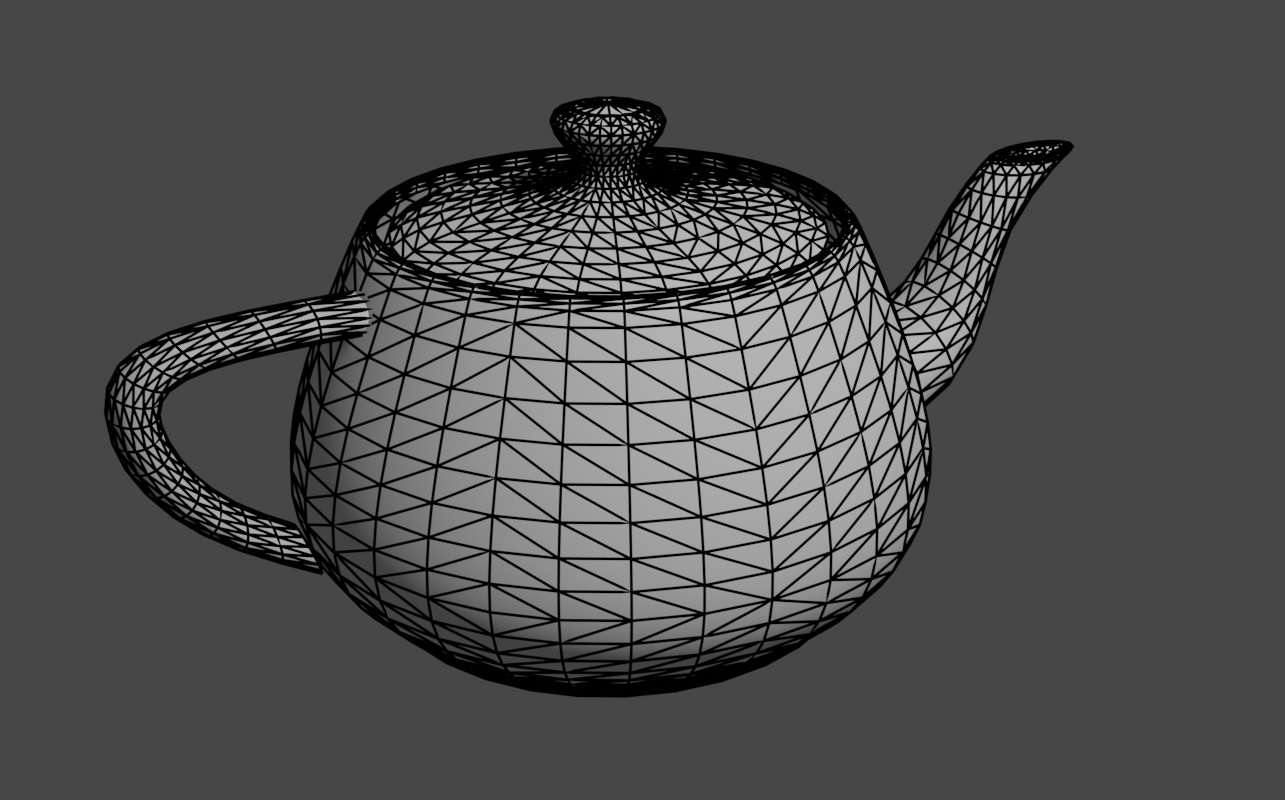
\includegraphics[width=.8\linewidth]{img/1 fundamentals/poly_mesh.png}
	\caption{Polygon mesh of the famous Utah Teapot, rendered with Blender \cite{blender2018}}
	\label{fig:poly_mesh}
\end{figure}

Various ray primitive intersection algorithms exist, for example, the Möller-Trumbore intersection algorithm \cite{moller1997fast} for intersecting triangles. To test a given ray for intersection with a polygon mesh, in theory, all polygons contained in the mesh in question must be tested for intersection. This is, of course, a naive and costly approach since the number of intersection tests that need to be performed is linear in the number of polygons. As such, polygon meshes are often composed of several thousand polygons, and testing them all for intersection has a decisive influence on the performance of the rendering process. Section \ref{sec:acceleration} introduces acceleration data structures, aiming at the minimization of those intersection tests.

\subsection{Constructive Solid Geometry (CSG)}
\todo{rewrite this whole section}
The core idea behind \emph{constructive solid geometry (CSG)} is the representation of more complex geometry by the application of Boolean set operations to a manageable amount of geometric primitives. The boolean set operators are union (logical \texttt{OR}), intersection (logical \texttt{AND}) and difference (denoted as \texttt{SUB}-operator).
Primitives are usually analytically described surfaces such as spheres, cones, and cylinders. However, polygon meshes can be used as primitives for CSG, too. Figure \ref{fig:csg} shows the application of each Boolean operator to two sphere primitives. Multiple applications of set operations with geometric primitives can be hierarchically ordered in a binary tree structure, called the CSG tree.   

\begin{figure} 
	\centering
	\subfloat[Union of two spheres (\texttt{OR} operator).]{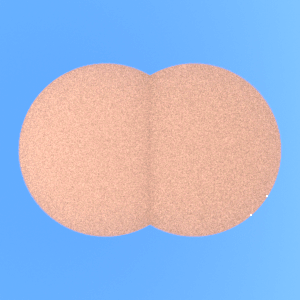
\includegraphics[width=.3\textwidth]{img/1 fundamentals/or.png}\label{fig:csg_or}}
	\hfill
	\subfloat[Intersection of two spheres (\texttt{AND} operator).]{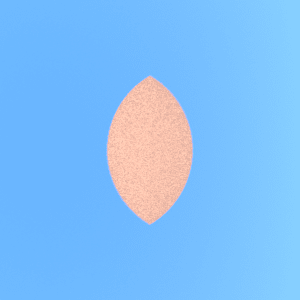
\includegraphics[width=.3\textwidth]{img/1 fundamentals/and.png}\label{fig:csg_and}}
	\hfill
	\subfloat[Left sphere with the right sphere "subtracted" from it (\texttt{SUB} operator).]{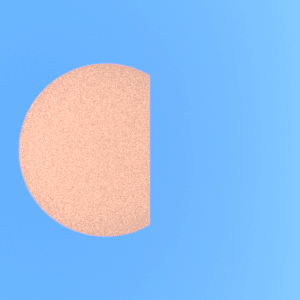
\includegraphics[width=.3\textwidth]{img/1 fundamentals/sub.png}\label{fig:csg_sub}}
	\caption{Boolean operators Union (\ref{fig:csg_or}), Intersection (\ref{fig:csg_and}) and Difference (\ref{fig:csg_sub}) applied to two sphere objects.}
	\label{fig:csg}
\end{figure}

One example of such CSG tree is provided in Figure \ref{fig:csg_tree}. Its leaves are associated with the geometry primitives, its interior nodes with a set operation. Due to the possibility that two primitives can be translated, rotated, or scaled before a Boolean operator is applied to them, the edges of the tree can be associated with transformation information (this is indicated in Figure \ref{fig:csg_tree} with the matrix icon) if a transformation is applied to the primitives \todo{reformulate}

\begin{figure}
	\centering
	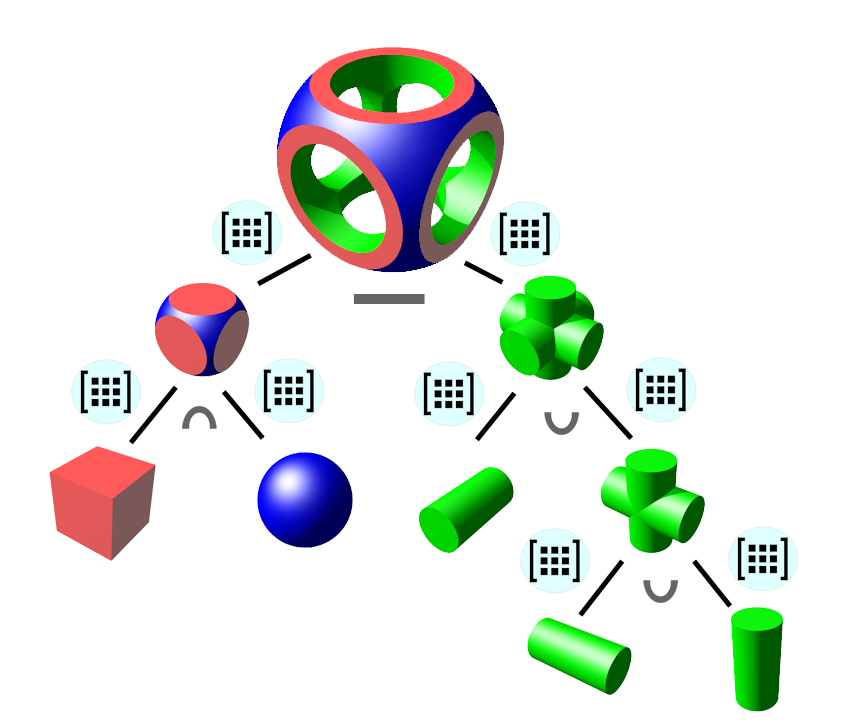
\includegraphics[width=.9\linewidth]{img/1 fundamentals/csg_tree.png}
	\caption{Visualization of a CSG tree hierarchy, originally created by \cite{csgtree} and updated
	with a matrix icon symbolizing affine transformations of geometries.}
	\label{fig:csg_tree}
\end{figure}

\subsubsection{Ray tracing with CSG}

\begin{figure} 
	\centering
	\subfloat[Union of two spheres (\texttt{OR} operator).]{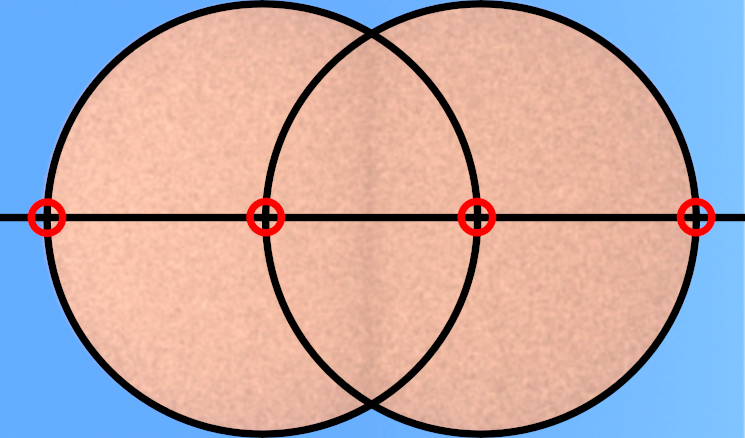
\includegraphics[width=.4\textwidth]{img/1 fundamentals/CSGall.png}\label{fig:csg_all_rc}}
	\hfil
	\subfloat[Intersection of two spheres (\texttt{AND} operator).]{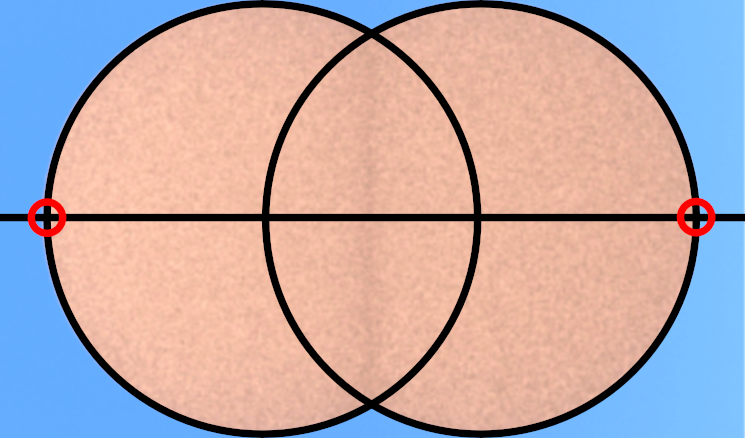
\includegraphics[width=.4\textwidth]{img/1 fundamentals/CSGor.png}\label{fig:csg_or_rc}}
	\\
	\subfloat[Left sphere with the right sphere "subtracted" from it (\texttt{SUB} operator).]{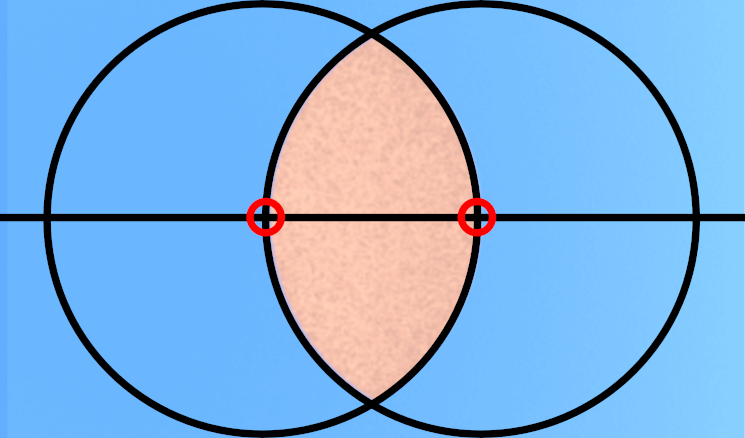
\includegraphics[width=.4\textwidth]{img/1 fundamentals/CSGand.png}\label{fig:csg_and_rc}}
	\hfil
	\subfloat[Left sphere with the right sphere "subtracted" from it (\texttt{SUB} operator).]{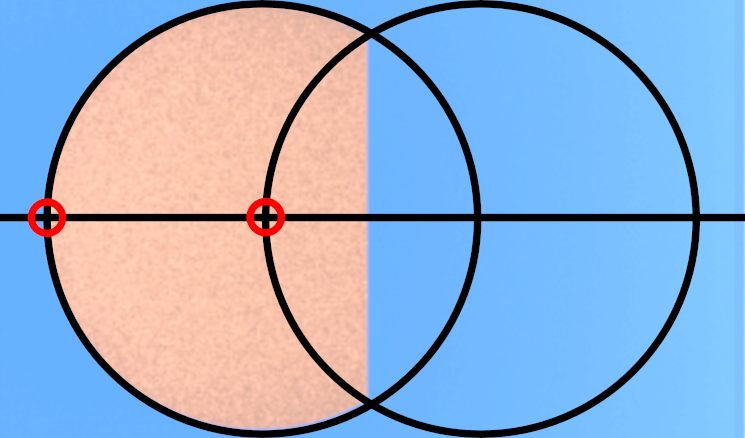
\includegraphics[width=.4\textwidth]{img/1 fundamentals/CSGsub.png}\label{fig:csg_sub_rc}}
	\caption{I will think of a caption later...}
	\label{fig:csg_rc}
\end{figure}

The ray tracing of CSG was pioneered by \cite{roth1982ray}. In the algorithm described in this \todo{do}, the intersection calculation for a given ray during the ray tracing process is straightforward: 
All the primitives associated with the leaves of the CSG tree are tested for intersection. If an intersection test with a quadric shape for instance has a positive result, usually two intersection points are calculated: one point when the ray enters the primitive and one point when it exits it (there is the edge case that there exists infinitely many intersection points between a ray and a primitive when the ray is tangent to the primitive, however, this is seldom the case and can be safely ignored). \todo{fucking fix this sentence}Then the CSG tree is traversed bottom up, and each time an interior node, representing a boolean set operator, is encountered, the intersection points of the ray with the primitives associated with the child nodes are evaluated and re-arranged. For example, when considering the \texttt{OR} operator in Figure \ref{fig:csg_or}, and given that a single ray would intersect both spheres, there would be four intersection points: One entering the first sphere, followed by one entering the second sphere, then one exiting the first sphere, and finally one intersection point exiting the second sphere. The \texttt{OR} operator would treat the two spheres as one single object and therefore discard the interior intersection points. Similarly, the \texttt{AND} operator in Figure \ref{fig:csg_and} would discard the two intersections at the exterior of the spheres and keep the two intersections contained in both spheres.
And finally, the \texttt{SUB} operator in Figure \ref{fig:csg_sub} discards every intersection point on the sphere (exterior or interior) that is "subtracted" from the sphere on the left.
\todo{fucking fix this explanation}

The representation of CSG offers one significant advantage: Complex geometry can be expressed via the composition of a manageable amount of primitive shapes, as opposed to large numbers of polygons in a polygon mesh. Because testing whether a point lies inside or outside a primitive is easy, as noted in Section \ref{sec:quadrics}, and since the number of primitives of a composed CSG is usually lower than the amount of polygons in a polygon mesh, the number of intersection tests in each render pass is comparatively low.

Although the CSG modeling technique is several years old, it is still used in practice today, e.g. for computer-aided design.


\section{Spacial acceleration data structures} \label{sec:acceleration}
The computational cost associated with ray tracing and path tracing algorithms has always been regarded as a "necessary evil" one faces when desiring highly realistic images. An often-cited fact is Whitted's observation that, for complex scenes, 95 percent of the time used by his algorithm is spent on intersection calculations \cite[p 349]{whitted1979improved}. To give an example, the image displayed in Figure \ref{fig:kajiya_figure} was rendered via path tracing on an IBM 3081 machine during 1221 minutes \cite[p 149]{kajiya1986rendering}. The image had a resolution of 512 by 512 pixels and was rendered with 40 paths per pixel.

It was only a logical consequence that new ideas were introduced over time, aiming at accelerating the ray tracing process. Be it through the minimization of the number of rays cast into the scene, the development of faster intersection testing algorithms, or the minimization of ray-primitive intersection tests. \emph{Acceleration data structures} are intended to reduce the number of unnecessary intersection calculations. By utilizing these structures, one essentially trades a decrease of the time needed to perform intersection testing to increase storage space. The following section focuses on two popular acceleration data structures commonly used: Bounding volume hierarchies and KD trees.

\subsection{Bounding Volume Hierarchies}

\emph{Bounding Volume Hierarchies (BVHs)} are hierarchical structures of so-called \emph{bounding volumes}, aiming at the reduction of unnecessary intersection tests. Bounding volumes enclose geometries with an analytical shape, such as a sphere, a cylinder, or a box. As previously discussed in Section \ref{sec:quadrics}, testing for an intersection between a given ray and one such analytical shape is easy. If no intersection with such volume is found, it is logical that an intersection between the ray and the enclosed geometry is not possible. Therefore, the intersection calculation between the ray and the enclosed geometry can be safely disregarded. 

\begin{figure}
	\centering
	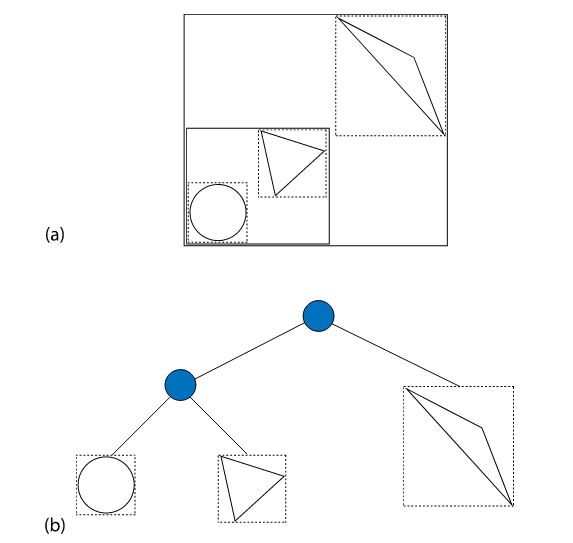
\includegraphics[width=.7\linewidth]{img/1 fundamentals/bvh.png}
	\caption{2D example of a bounding volume hierarchy, taken from \cite{pharr2016physically}. (a) represents the scene, consiting of simple shapes and their axis aligned bounding boxes and (b) the BVH tree structure associated with the scene from (a).}
	\label{fig:bvh}
\end{figure}

Bounding volumes should ideally be chosen to fit the underlying geometry as close as possible to reduce the number of unnecessary intersection tests further. However, a most commonly used volume is an \emph{axis aligned bounding box}, a hyperrectangle whose sides are parallel to the axis of the coordinate system. Such boxes might not enclose the geometry as tightly as possible. On the other side, testing for intersections becomes computationally cheap, and not much memory is needed to store them.

Again, these bounding volumes can be enclosed in a bounding volume, and thus, complex hierarchies of bounding volumes can be formed.
A BVH then is a hierarchy of multiple of such bounding volumes stored in a tree structure. The leaves of the tree represent the bounding boxes of the geometry contained in the scene, and the interior nodes are associated with bounding volumes enclosing the node's children. The bounding box associated with the tree root encloses the entire scene. An example of such a tree structure is given by Figure \ref{fig:bvh}.

Binary BVHs exhibit some convenient properties: \todo{fucking, check this dude! could be plain wrong} Every geometrical primitive is present in exactly one bounding box, and these bounding boxes do not overlap with each other. Thus, no primitive is possibly tested for intersection twice (unlike with KD trees, which are the subject of the next section). Furthermore, the amount of memory needed for storing a binary BVH is bounded. 

A BVH that is build over $n$ primitives obtains $2n-1$ total nodes, $n$ leave nodes and $n-1$ interior nodes, as noted in \cite{pharr2016physically}.

During ray tracing, the BVH is traversed, and a cast ray is tested for intersections between a bounding box associated with the current tree node. If an intersection is found, the traversal continues in the node's children, otherwise traversing the subtree rooted at that node is disregarded.


\subsection{KD Trees}

\begin{figure}
	\centering
	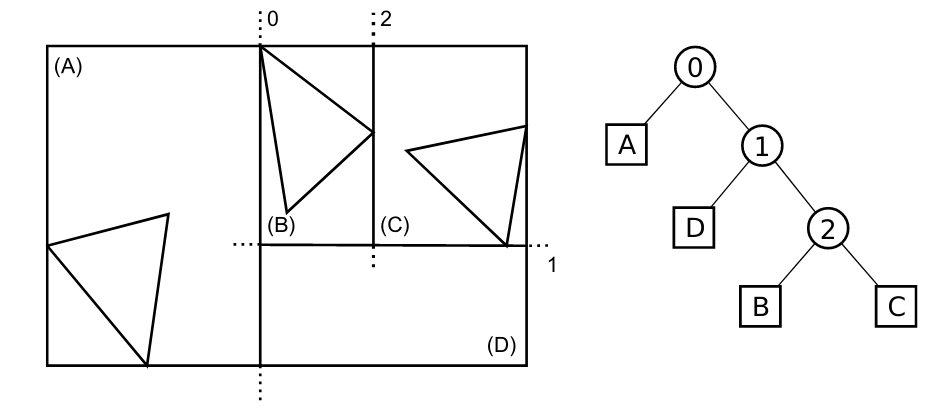
\includegraphics[width=1\linewidth]{img/1 fundamentals/kd_tree.png}
	\caption{Partition of a 2D scene in sub spaces A, B, C, and D with planes 0, 1, and 2. This figure is taken from \cite{hapala2011kd}.}
	\label{fig:kdtree}
\end{figure}

\emph{K-dimensional trees} (or KD trees), which were introduced by \cite{bentley1975multidimensional}, belong to the group of \emph{binary space partitioning trees (BSP trees)}. BSP trees recursively subdivide $k$ dimensional space with $k-1$ dimensional hyperplanes. One subdivision of space occurs when the number of geometric primitives contained in it is greater than a specified threshold. When one such subdivision takes place, space is divided into two smaller half-spaces. This procedure is repeated for each of the two half-spaces until the number of primitives contained in a subdivided area is smaller or equal to the threshold. The hyperplanes that partition space are stored in a tree structure. The root of the tree is associated with the hyperplane splitting the bounding volume of the entire scene. Its children to the left are the hyper-planes and primitives in one half-space, and the children to the right are the planes and primitives located in the other half-space. The leaf nodes correspond to a list of primitives located in the area bounded by the hyper-planes associated with their parent nodes in the tree.

KD trees are a specialized case where the split-planes are perpendicular to one of the coordinate axis. During the recursive splitting, the axis to which the current plane is perpendicular to, is alternated. This allows for KD trees being efficiently constructed. However, \todo{check this too!} unlike with BVHs, primitives can be located in overlapping sub spaces, therefore intersection points may be calculated twice during ray tracing. 

Construction methods taking $O(n\log n)$ time exists \cite{wald2001interactive}.) \todo{re-write}

\section{Intel's Embree framework}
Despite the effect of various ray acceleration data structures and hardware optimizations, exploiting the full capabilities of modern CPUs, which exhibit different architectures and instruction sets and support different algorithms and data structures, remains challenging for ray tracing applications.

Embree is a high performance rendering framework written in C99 which addresses this problem. It offers a collection of vectorized kernels optimized for communication with CPUs that support SSE, AVX, AVX2, AVX-512, and instruction sets. The provided kernels offer a variety of components, e.g., different types of BVHs, traversal algorithms, and intersection algorithms, Figure \ref{fig:embree} provides an overview.
During a rendering process, Embree will decide on which components to use for building the acceleration structure and traversing it based on information provided by the user and on the target CPU architecture. The latter is performed by the "Ray Tracing Kernel Selection" layer of the hierarchy shown in Figure \ref{fig:embree}.

Interesting features of Embree are:
\begin{itemize}
	\setlength\itemsep{0.05em}
	\item 	Finding of the closest hit point, or alternatively any hit point,
	\item 	support for the cast of single rays, ray packets containing 4, 8 or 16 rays, and so-called ray streams of any desired number of rays,
	\item 	high-quality BVH builders,
	\item 	support for the Intel SPMD Program Compiler (ISPC) and the Intel Threading Building Blocks (TBB), and
	\item 	independence from any other graphics API such as OpenGL or DirectX
\end{itemize}

An API for the integration into existing rendering systems is provided and described in a detailed documentation \cite{embree2021Doc}. This documentation furthermore offers a tutorial for the familiarization of the framework to new users. The name of the functions belonging to this API are preceded by the abbreviation \texttt{rtc} ("ray tracing kernels"), data types have the abbreviation \texttt{RTC} predeceasing their name. For example the variable \texttt{RTCScene} stores the virtual scene for Embree, and the function \texttt{rtcIntersect1} performs the intersection testing with a single ray.

\begin{figure}
	\centering
	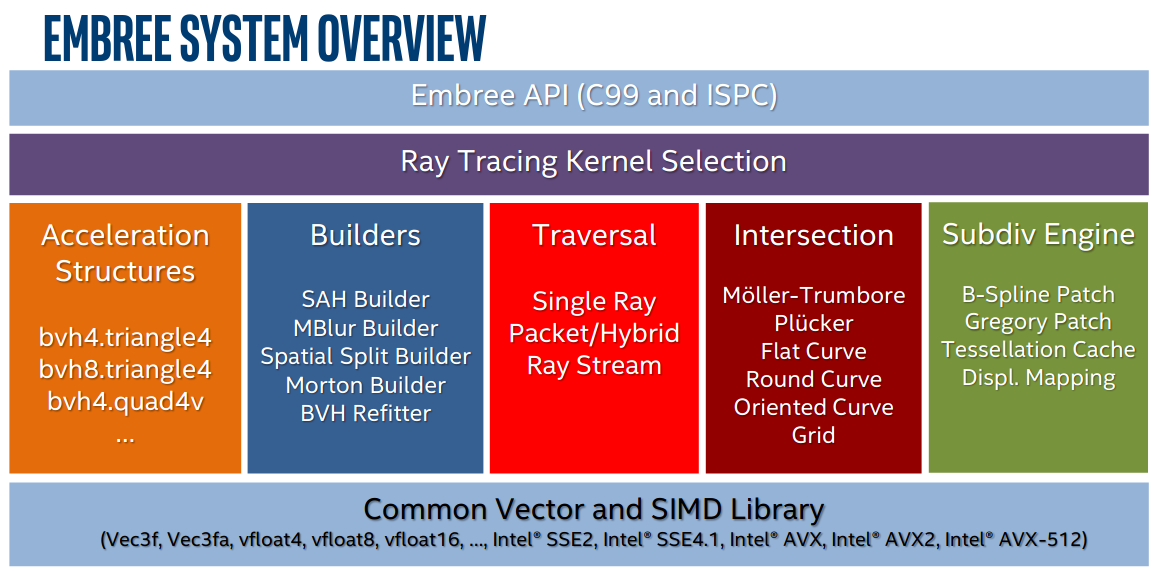
\includegraphics[width=1\linewidth]{img/1 fundamentals/embree_overview.png}
	\caption{System overview of Embree. This figure is a slide from the SIGGRAPH presentation \citetitle{embreeSlides} \cite{embreeSlides}.}
	\label{fig:embree}
\end{figure}

Embree supports various geometric shapes such as triangles, quads, and certain types of curves, such as Bézier curves, B-Splines and Catmull-Rom-Splines.
Another notable feature of Embree is the support of custom geometries of the rendering system it is integrated into. These will be referred to as \emph{User defined geometries}.

Embree is open source and therefore publicly available. Supported platforms are (32-bit and 64-bit), Linux (64-bit), and macOS (64-bit). The latest version of Embree at the time of writing this thesis is 3.13.0. 